\documentclass[11pt, fleqn]{article}

\documentclass[11pt, fleqn]{article}

\usepackage[usenames,dvipsnames,svgnames,table]{xcolor}
\usepackage{amsmath}
\usepackage{amsfonts}
\usepackage[margin=1in]{geometry} % To set the margin widths
\usepackage{graphicx}
\usepackage{listings}
\usepackage{multirow}
\usepackage{tabularx}
\usepackage{varioref}
\usepackage[noabbrev,capitalize]{cleveref}
\usepackage[group-separator={,}]{siunitx}
\usepackage{subcaption}
\usepackage{titlesec}
\usepackage{lscape}
\usepackage{bm}
\usepackage[titletoc,toc,title]{appendix}

\lstset{
  frame=single,
  basicstyle=\ttfamily,% print whole listing small
  language=R,
  aboveskip=3mm,
  belowskip=3mm,
  showstringspaces=false,
  columns=flexible,
  numbers=none,
  commentstyle=\color{ForestGreen},
  stringstyle=\color{Maroon},
  breaklines=true,
  breakatwhitespace=true,
  tabsize=2,
  literate={<-}{{$\gets$}}1 {~}{{$\sim$}}1
}

\sisetup{output-exponent-marker=\textsc{e}}

\setlength{\parskip}{12pt} % Sets a blank line in between paragraphs
\setlength\parindent{0pt} % Sets the indent for each paragraph to zero

% \crefname{figure}{Figure}{Figures}
% \crefname{section}{Section}{Sections}
% \crefname{table}{Table}{Tables}
% \crefname{lstlisting}{Listing}{Listings}

\setlength{\parskip}{12pt} % Sets a blank line in between paragraphs
\setlength\parindent{0pt} % Sets the indent for each paragraph to zero

\begin{document}

\title{Machine Learning (41204-01)\\HW \#3}
\author{Will Clark $\vert$ Matthew DeLio \\
\texttt{will.clark@chicagobooth.edu} $\vert$ \texttt{mdelio@chicagobooth.edu} \\
University of Chicago Booth School of Business}
\date{\today}
\maketitle

\section{Data}

For this exercise, our data set contains the sale price and the observable characteristics for a sample of 20,000 used cars. We randomly sampled it to break this data into three subsets: 50 percent of data will be our training set that will be used to train/tune our models ($n=10,031$); 25 percent will be our validation data set which we will use to evaluate model performance ($n=5,016$); and 25 percent will be our test set which we will use to evaluate out-of-sample performance of our best model ($n=5,016$).

We will build a series of models that can predict the selling price of a used car given its observable characteristics. The models and techniques we will use are: (1) regression trees, (2) bagging, (3) random forests, and (4) boosting trees.

\section{Regression Trees}

We begin by fitting a simple regression tree to the data. We use the \texttt{rpart} package on the training data set discussed above. The \texttt{rpart} method returns an object that includes a matrix of the optimal tree prunings. We use this matrix to find the tree complexity parameter that produces the lowest error and prune the tree to this level of complexity. The original tree and pruned tree for a small model (i.e. price on mileage) are depicted in \cref{fig:tree_small} and \cref{fig:tree_small_prune}, and it is clear that the pruned model has fewer end nodes than the original model.

Because the default options on \texttt{rpart} choose a very simple tree, we lower the minimum split (i.e. smallest number of observations in a node in order for it to be split) from 20 to five, and we lower the complexity parameter from 1/100 to 5/10,000 (which effectively builds more splits into the tree). This produces a more complex model, but one that still does not perform well out-of-sample, especially in comparison to the other algorithms discussed below.

\begin{figure}
  \centering
  \begin{subfigure}[b]{0.49\textwidth}
 \caption{Small Regression Tree}
 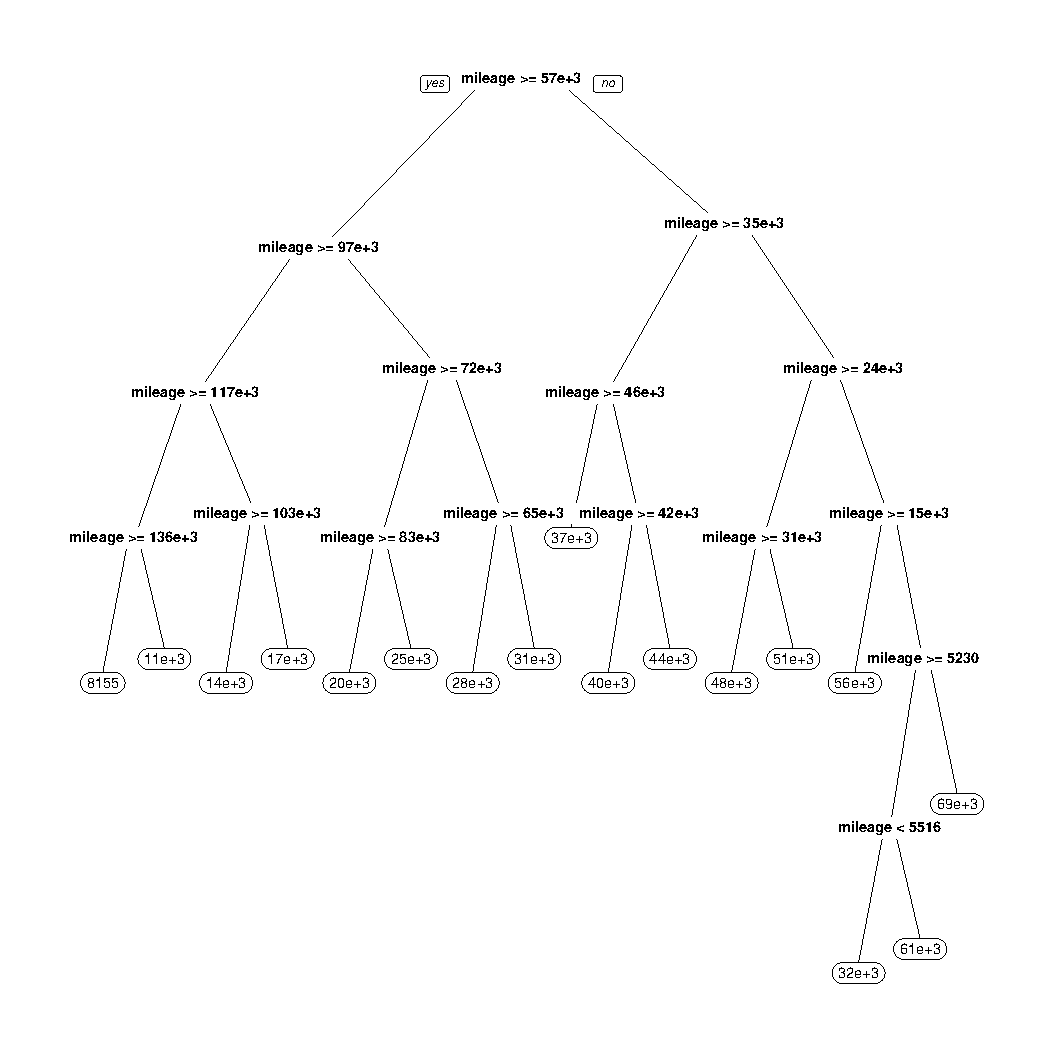
\includegraphics[width=\textwidth]{tree_small.pdf}
 \label{fig:tree_small}
  \end{subfigure}
  \hfill
  \begin{subfigure}[b]{0.49\textwidth}
 \caption{Small Regression Tree (Pruned)}
 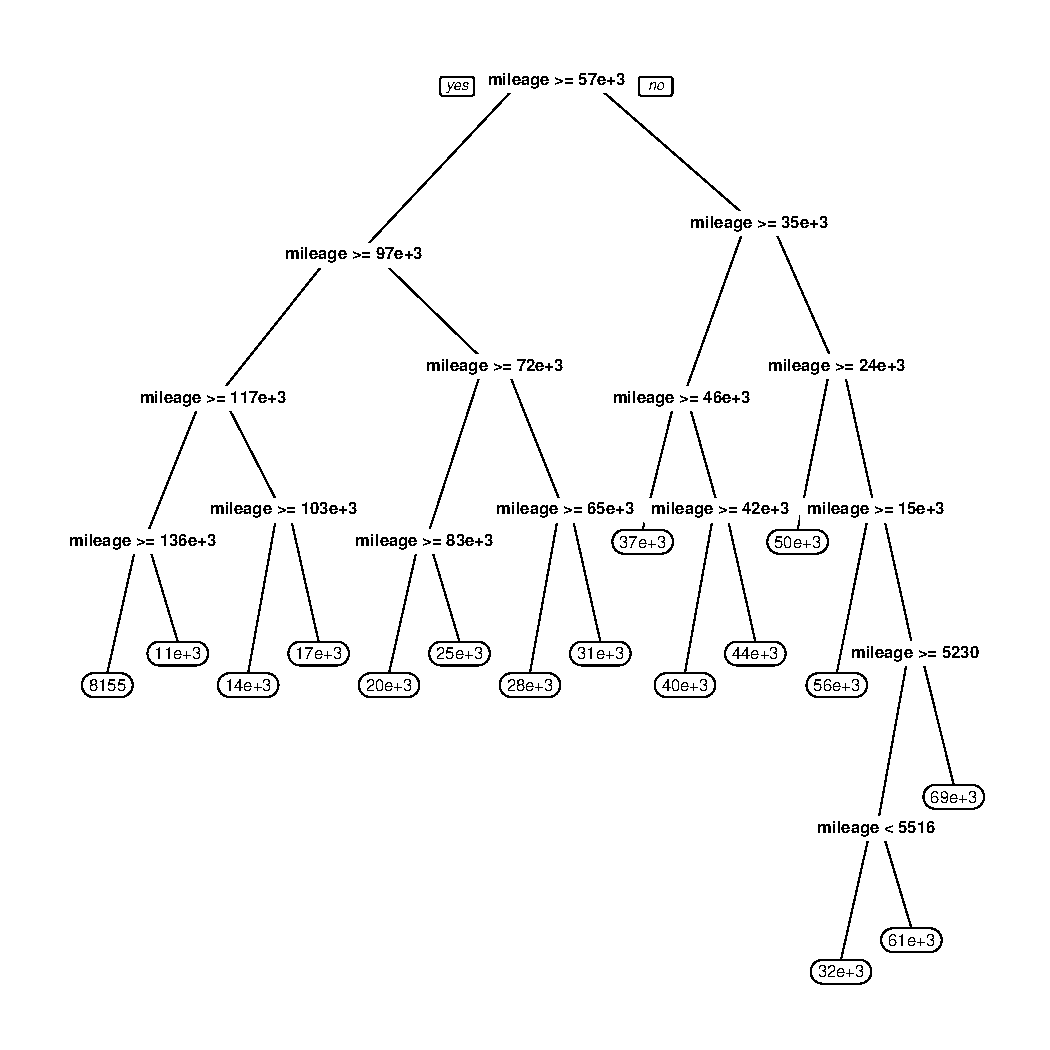
\includegraphics[width=\textwidth]{tree_small_prune.pdf}
 \label{fig:tree_small_prune}
  \end{subfigure}
 \caption{Comparison of Small Regression Tree Models}
\end{figure}

\section{Bagging}

In this section, we use an aggregate bootstrap technique to predict used car sales price. The basic algorithm is:
\begin{itemize}
\item For a given number of trials $T$:
\begin{itemize}
\item Select a bootstrap sample from the data and fit a large regression tree on this sample (in this case we take large to mean a tree that is not pruned);
\item Use the large tree to make a prediction for expected price;
\end{itemize}
\item Take an average of the predicted price across all trials.
\end{itemize}

Ultimately, the bagging algorithm does not perform very well relative to the boosting tree, the random forest, and the LASSO regression. 

\section{Random Forest}

In this section, we try to predict car price with a random forest algorithm. The main difference between the algorithm here and that in the prior section is that for each tree, instead of estimating based on the entire set of covariates, we estimate only on a subset $m$ of covariates. This makes the algorithm train more quickly and introduces another layer of randomness into our predictions. 

We chose a value of $m=3$, which produced the best set of out-of-sample RMSE values. We also chose to stop the algorithm after 250 trees, as the predictive performance (measured by out-of-bag RMSE) fails to improve after this point (see \cref{fig:rf_oob_mse}). In order to speed up performance even more, we can also divide our intended number of trees (250) by the number of processors available (eight, in this case). We then build each small forest on a separate processor, combine the eight forests at the end into one larger forest and use this final combined forest to predict car price.

The random forest algorithm ends up performing very well, nearly beating the best-in-class performance of the boosting tree.

\begin{figure}[!htb]
  \centering
  \caption{Out-of-Bag Mean Square Error by Number of Trees}
  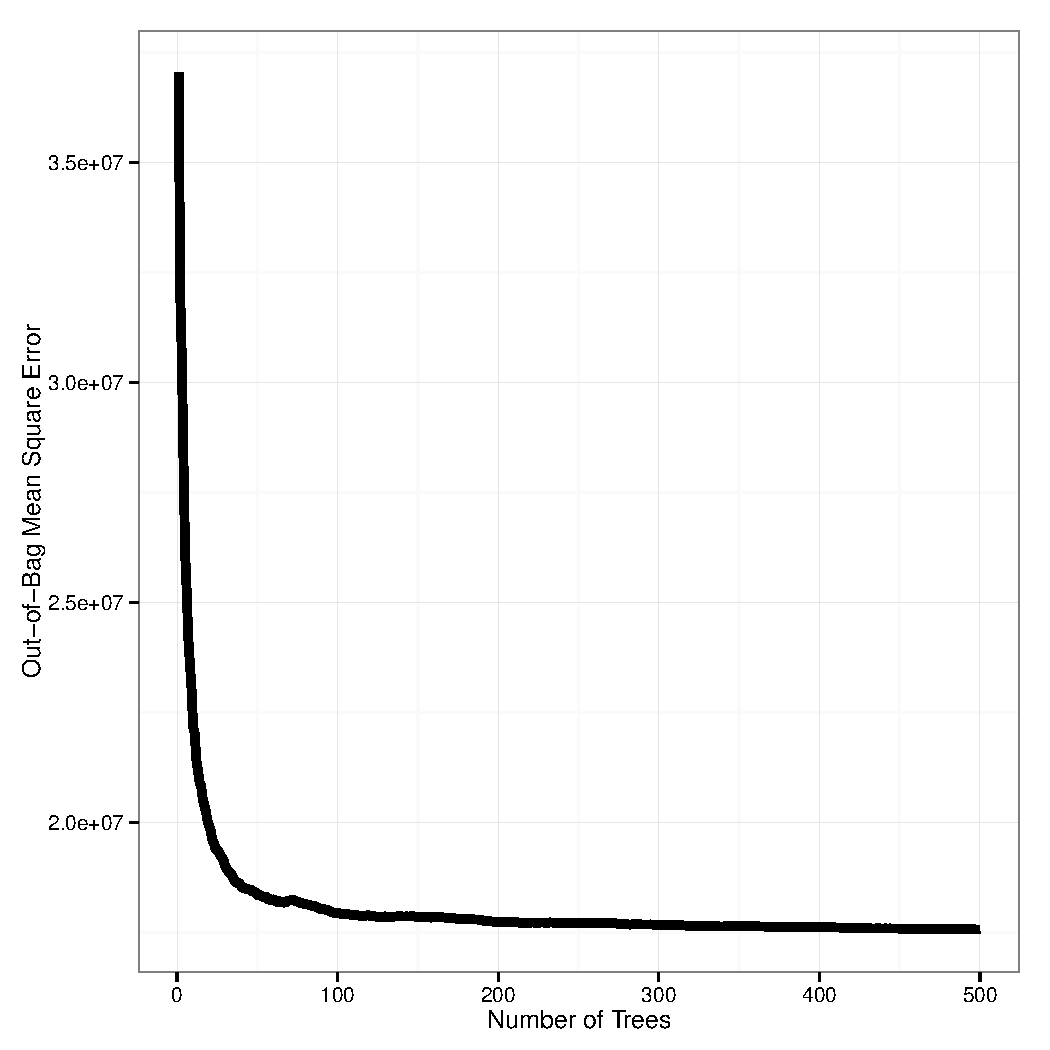
\includegraphics[scale=.5]{rf_oob_mse.pdf}
  \label{fig:rf_oob_mse}
\end{figure}

\section{Boosting Trees}


\section{LASSO Regression}

\section{Comparison and Out-of-Sample Test}

In \cref{tab:rmse_comp}, we list the out-of-sample RMSE of each model for the validate data set. The models denoted by ``large'' are those trained on the entire set of covariates; those denoted by ``small'' are trained only on the mileage series.

The best performing model is the large boosting tree model, followed very closely by the large random forest model and the large LASSO regression model. All three models perform similarly, although the boosting tree model was the most difficult to tune. In a production environment, deciding which model is best would depend not only on performance but on computational expense. Because the three models mentioned above all perform so closely, we will test all three on the out-of-sample test set and see how they perform.

The results of the out-of-sample test are shown in \cref{tab:rmse_test}. Two things are clear. The first is that the \textit{true} out-of-sample RMSE for all three models is very close to our expected out-of-sample RMSE based on the validation data set. The second is that the order of performance of the models is now different: the random forest actually predicted better in the true out-of-sample test than the boosting tree did. This suggests that at the margin, we can differentiate what is the ``best'' model by other factors like tractability and computational expense, and out-of-sample performance will not suffer much as a result.

% latex table generated in R 3.2.1 by xtable 1.7-4 package
% Thu Oct 15 03:45:24 2015
\begin{table}[ht]
\centering
\caption{Comparison of RMSE for Various Models} 
\label{tab:rmse_comp}
\begin{tabular}{lr}
  \hline
Model & RMSE \\ 
  \hline
Boosting Tree (big) & 2895.43 \\ 
  Random Forest (big) & 2965.92 \\ 
  LASSO Regression (big) & 3200.54 \\ 
  Bagging (big) & 3407.65 \\ 
  Regression Tree (big) & 3407.65 \\ 
  Pruned Regression Tree (big) & 4588.53 \\ 
  Boosting Tree (small) & 7248.59 \\ 
  Bagging (small) & 7292.48 \\ 
  Regression Tree (small) & 7292.48 \\ 
  Pruned Regression Tree (small) & 7512.58 \\ 
  Random Forest (small) & 8389.08 \\ 
   \hline
\end{tabular}
\end{table}


% latex table generated in R 3.2.1 by xtable 1.7-4 package
% Thu Oct 15 03:48:17 2015
\begin{table}[ht]
\centering
\caption{OOS RMSE for Top Three Models} 
\label{tab:rmse_test}
\begin{tabular}{lrr}
  \hline
Model & RMSE (Validate) & RMSE (Test) \\ 
  \hline
Boosting Tree & 2895.43 & 2858.09 \\ 
  Random Forest & 2965.92 & 2864.27 \\ 
  LASSO Regression & 3200.54 & 3097.48 \\ 
   \hline
\end{tabular}
\end{table}


\end{document}

% \input{.tex}

% \begin{figure}
%   \centering
%   \begin{subfigure}[b]{0.49\textwidth}
%     \caption{}
%     \includegraphics[width=\textwidth]{.pdf}
%     \label{fig:}
%   \end{subfigure}
%   \hfill
%   \begin{subfigure}[b]{0.49\textwidth}
%     \caption{}
%     \includegraphics[width=\textwidth]{.pdf}
%     \label{fig:}
%   \end{subfigure}
%   \caption{}
% \end{figure}

% \begin{figure}[!htb]
%   \centering
%   \caption{}
%   \includegraphics[scale=.5]{.pdf}
%   \label{fig:}
% \end{figure}

